En el presente trabajo se analizó, diseñó e implementó una aplicación web capaz de ofrecer a un usuario una herramienta para gestionar visualizaciones sobre ediciones de un artículo wiki. Como primer requerimiento el usuario tiene que crearse una cuenta para mantener una sesión privada, luego podrá agregar artículos principalmente de Wikipedia en idioma Español e Inglés, esto requiere que se active el proceso de extracción en el API de Wikimetrics para obtener las ediciones del mismo. Una vez extraído el artículo podemos acceder al detalle en donde encontraremos información específica y base como número de ediciones, número de ediciones menores, fecha de ultima edición, usuario de ultima edición, número de usuarios que editaron, tamaño de artículo y link al artículo de Wikipedia. Esta vista de detalle ofrece también la posibilidad de crear visualizaciones y una lista donde se muestran. Además, se presentará una lista de visualizaciones predeterminadas, entre ellas la que resalta es la gráfica Wiki History Flow. Las visualizaciones creadas por el usuario pueden habilitarse para mostrar su preview en una sección del mismo detalle de artículo, al presionar tanto el preview como la visualización del listado podemos entrar al editor de visualizaciones. En el editor de visualizaciones se nos presenta un selector en donde podemos definir el filtro, la vista y la agrupación, luego de esto tenemos un selector para definir el tipo de gráfica a visualizar. 

Para la construcción de la aplicación nos apoyamos del framework Angular y Angular Material para el diseño, fue necesario usar el API de Wikipedia para ofrecer las sugerencias de artículos en la creación del mismo. Para las visualizaciones extraemos los datos del API de Wikimetrics y nos apoyamos de las bibliotecas D3 y Plotly para graficarlas de manera fácil.

\begin{center}
    \bigbreak
    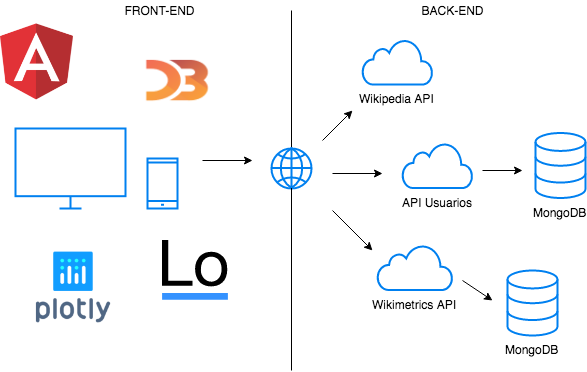
\includegraphics[scale=0.45]{images/conclusiones/tech_context.png}
    \captionof{figure}{Esquema abstracto de las tecnologías involucradas en el trabajo}
    \label{fig:library_comparison}
    \bigbreak
\end{center}


\section{Contribuciones}
\begin{itemize}
    \item Se realizó una investigación amplia de bibliotecas de visualización que puede servir como apoyo para la decisión de futuros trabajos dependiendo de los requerimientos.
    
    \item Se realizó investigación en el área de Visualización de Datos, refrescando conceptos teóricos claves y planteamientos de como resolver problemas haciendo uso de diferentes técnicas.
    
    \item Se implementó un componente en Angular que facilita la creación de visualizaciones responsives usando Plotly, en donde será de apoyo para aquellos trabajos que involucren las mismas tecnologías.
    
    \item Se elaboró un componente de Angular que construye la gráfica Wiki History Flow haciendo uso de D3. Para trabajos futuros puede servir de apoyo para la mejora o construcción de la misma.
    
    \item Al ser una aplicación web que implica tecnologías nuevas e interesantes puede aportar contenido y ejemplos para la materia de Aplicaciones en Internet.
\end{itemize}

\section{Limitaciones}

\begin{itemize}
    \item Principalmente se iba a usar el API de Wikipedia para realizar la autenticación de usuarios y extraer los artículos de su watchlist como primera instancia, pero Wikipedia dejó obsoleta la manera vieja de autenticación y la nueva forma es mediante OAuth2, por lo que pedían usa serie de requerimientos que estaban fuera del alcance. Por tal motivo se optó por gestionar los usuarios con nuestro propio sistema.
    
    \item Para la realización de visualizaciones se tuvo que diseñar e implementar un nuevo end-point en el API de Wikimetrics debido a que los otros eran pocos flexibles. Por lo tanto se tomó tiempo del trabajo para el análisis de la misma. Con el nuevo end-point por falta de tiempo los queries en mongo los tuvo que definir el front-end en base a los requerimientos.
\end{itemize}

\section{Trabajos futuros}

\begin{itemize}
    \item Dejar de manejar los usuarios internamente y manejar la autenticación con el API de Wikipedia. Lo principal sería cumplir con los requerimientos que pide MediaWiki como API para crear la aplicación usando OAuth2. De esta forma solo manejaremos un inicio de sesión usando el usuario de Wikipedia.
    
    \item Habilitar una opción para poder sincronizar los artículos del watchlist del usuario de Wikipedia con los artículos de esta plataforma.
    
    \item Analizar qué visualizaciones pueden ser frecuentes en los usuarios y ofrecerlas como visualizaciones predeterminadas.
    
    \item Implementar la gráfica original de History Flow. Esta visualización requiere de mucho cómputo, por lo que calcularlas en el front-end es inviable. La idea es delegarle esta funcionalidad a un servicio en el back-end que envíe los datos preparados para la visualización.
    
    \item Alguna funcionalidad para compartir dashboard de visualizaciones o visualizaciones individuales en modo de solo lectura
\end{itemize}